\chapter{Controlling Weakly-coupled Carbon Spins}
[Note intro needs to be rewritten once chapter is done]\\
Now that we have identified several promising carbon spins we will go into controlling them.
This chapter attempts to explain first how we can control a carbon by explaining how the two different rotation axes from the last chapter can be used to implement a conditional +-X gate. A gate similar to a CNOT gate.
Now that we understand how to implement a cnot gate we will use this to perform an experiment that we call a carbon ramsey on an unitialized state.
AFterwards we will use this to show that we can initialize and readout by showing an initialized carbon ramsey. (1buit tomo (ramsey with more T +Z-RO?).
From this we will also determine $T_{2 \mathrm{C}}^*$.

The next section will consider two qubit control.
It will start by explaining how we can perform a parity measurement. This measurement allows us to perform a two qubit tomography and create entanglement by projection.
We will then show

\section{Controlling a single-carbon}
This section will explain how a weakly-coupled spin can be controlled using the conditional rotation of the carbon spin that occurs when on resonance (\cref{eq:res_dip_loc}).
It will start by explaining how to do basic gate operations in the ideal case of being perfectly on resonant and not interacting with any nuclear spins.
After that we will explain how a carbon-spin in a mixed state can be initialized

\subsection{Basic gates}
As was explained in \cref{sec:controllingacarbonthroughdynamicaldecoupling} nuclear spins perform a rotation along two anti-parallel axes when subjected to a dynamical decoupling sequence on a resonant condition given by \cref{eq:res_dip_loc}.
The angle of rotation can be controlled by choosing the number of pulses of the decoupling sequence.

By choosing the number of pulses such that all coherence is lost when performing a dynamical decoupling spectroscopy measurement on the resonance, a rotation of $\pi/2$ in the clockwise direction is performed when the electron is in the $\ket{0}$-state and a $\pi/2$-rotation in the counterclockwise direction when the electron is in the $\ket{1}$-state.
We define the axis of rotation of this operation as the X-axis.

We call this conditional rotation the $\pm \mathrm{x}$-gate and it forms the basis of our control over weakly coupled spins. \Cref{fig:gate_circuit_pm-x} shows how we depict the $\pm \mathrm{x}$-gate in a circuit-diagram.
By letting the phase of the carbon evolve we are able to apply operations on the carbon-spin with arbitrary phase.
An unconditional gate can be implemented by placing the electron in an eigenstate before performing the $\pm\mathrm{x}$-operation.

\begin{figure}[htbp]
    \centering
        \mbox{
        \Qcircuit @C=1em @R=.7em {
         \lstick{\ket{\Psi}_e} &\ctrl{1}  &\qw\\
          \lstick{\ket{\Psi}_\mathrm{C}} &\gate{\pm \mathrm{x} }  &\qw}}
    \caption{The conditional x-gate ($\pm\mathrm{x}$). Performs an x-rotation on the carbon state ($\ket{\Psi }_\mathrm{C}$) when the electron is in the $\ket{0}_e$-state. It performs a $-\mathrm{x}$ rotation when the electron is in the $\ket{1}_e$-state.}
    \label{fig:gate_circuit_pm-x}
\end{figure}

\subsection{Initializing a carbon-spin}
The $\pm\mathrm{x}$-gate can be used to initialize a carbon-spin.
To initialize a carbon-spin  in the $ \ket{X}$-state the gate-circuit as depicted in \cref{fig:gate_circuit_mbi_x-init} is implemented.

After the electronic-spin is brought in the $\ket{X}$-state the two-qubit system can be described by the tensor product of two density matrices:
\begin{equation}
    \rho_X \otimes \rho_m = \rho_X \otimes \rho_{X} +\rho_X \otimes \rho_{-X}
\end{equation}
By applying the $\pm{\mathrm{x}}$-gate  the electronic-spin picks up a phase depending on the nuclear spin-state:
\begin{equation}
     \rho_Y \otimes \rho_{X} +\rho_{-Y} \otimes \rho_{-X}
    \label{eq:density_after_Ren}
\end{equation}

The effect of the $\pm{\mathrm{x}}$-gate can be made more easily understood by treating the carbon-spin as being either in the $\ket{X}$ or $\ket{-X}$-state. Treating both as separate cases below.
\begin{align}
    \quad &\ket{X}\ket{X} &\vee \quad &  \quad\ket{X}\ket{-X}\\
    \quad &\frac{\ket{0}+\ket{1}}{\sqrt{2}}\ket{X} &\vee \quad & \quad \frac{\ket{0}+\ket{1}}{\sqrt{2}}\ket{-X} \\
    \quad &\frac{e^{-i\pi/4}\ket{0}+e^{i\pi/4}\ket{1}}{\sqrt{2}}\ket{X} &\vee \quad & \quad \frac{e^{i\pi/4}\ket{0}+e^{-i\pi/4}\ket{1}}{\sqrt{2}}\ket{-X}\\
    \quad &\ket{Y}\ket{X} &\vee \quad & \quad \ket{-Y}\ket{-X}
\end{align}
The final x-pulse is used to read out the electron. By conditionalizing the experiment on getting the outcome $\ket{0}_e$ the carbon is initialized in the $\ket{X}_C$-state.
\begin{equation}
    \rho_0 \otimes \rho_{\mathrm{X}} + \rho_1 \otimes \rho_{\mathrm{-X}}
\end{equation}

\begin{figure}[htbp]
    \centering
    \begin{subfigure}[t]{0.49\textwidth}
    \mbox{
        \Qcircuit @C=1em @R=.7em {
        \lstick{\ket{0}_e}                        & \gate{\mathrm{y}}  & \ctrl{1}       & \gate{\mathrm{x}} &\qw          &  \meter \\
        \lstick{\rho_\mathrm{m}}         & \qw              &  \gate{\pm \mathrm{x}}     & \qw    & \qw   & \qw}}
    \caption{MBI-based initialization into $\pm \ket{\mathrm{X}}$.}
    \label{fig:gate_circuit_mbi_x-init}
    \end{subfigure}
    \begin{subfigure}[t]{0.49\textwidth}
        \centering
        \mbox{
        \Qcircuit @C=1em @R=.7em {
            \lstick{\ket{0}_e} & \gate{\mathrm{y}}  & \ctrl{1} & \gate{\mathrm{x}} &\ctrl{1} &  \meter \\
            \lstick{\rho_\mathrm{m}}& \qw&  \gate{\pm \mathrm{x}}     & \qw    & \gate{\mp \mathrm{y}}    & \qw}}
        \caption{MBI-swap initialization.}
        \label{fig:gate_circuit_mbi_swap-init}
    \end{subfigure}
    \caption{\Cref{fig:gate_circuit_mbi_x-init} MBI-based initialization into $\pm \ket{\mathrm{X}}$. Initializes the carbon into $\ket{X}_\mathrm{C} $ when $\ket{0}_e$ is measured and into $\ket{-X}_\mathrm{C} $ when $\ket{1}_e$ is measured for the electron.
    \Cref{fig:gate_circuit_mbi_swap-init} MBI-swap initialization into $ \ket{\mathrm{0}}$. Initializes the carbon into $\ket{0}_\mathrm{C} $ regardless of the electronic spin-state measured.}
    \label{fig:gate_circuit_initialization}
\end{figure}

The sequence can be extended to a swap type initialization by implementing an additional $\mp{\mathrm{y}}$-gate.
The effect of the extra y-gate is that both the  $\ket{X}_\mathrm{C} $ and the  $\ket{-X}_\mathrm{C} $-state are rotated to the  $\ket{0}_\mathrm{C} $-state, effectively swapping the mixed state from the carbon to the electron.
By applying a readout the electron can be reinitialized.


\subsection{Carbon Ramsey experiment }
By performing a Ramsey experiment we can determine the precession of the carbon-spin and its dephasing-time $T_2^*$.
By determining the precession frequencies it is possible to track phase evolution and use that to implement operations with arbitrary phase.
By measuring the precession frequency it is also possible to disprove our estimation for the hyperfine parameters.
We require the dephasing time in order to determine if enough operations can be applied to implement quantum algorithms \footnote{Change this sentence}.

In an ordinary Ramsey experiment a qubit is brought to the equator of the Bloch-sphere where it precesses for a time $\tau $ before it is read out along the x-direction.
A carbon-Ramsey experiment is similar but slightly more complicated as the nuclear spin cannot be controlled and read-out directly.
An uninitialized and an initialized version are depicted in \cref{fig:gate_circuit_nuclear_ramsey}.

In the initialized version of the carbon-Ramsey experiment the system is first initialized in the $\ket{0}_e\ket{X}_\mathrm{C}$-state.
The carbon is let to precess for a time $\tau$ before the $\ket{X}_\mathrm{C}$-state is read out.
During the free evolution the carbon rotates with a frequency of $\omega_L$ because the electron is in $\ket{0}_e$ and there is no coupling between them.

\begin{figure}[htbp]
\begin{subfigure}[t]{\textwidth}
\centering
    \mbox{
    \Qcircuit @C=1em @R=.7em {
    \lstick{\ket{0}}          & \gate{\mathrm{y}}  & \ctrl{1}   &\gate{\mathrm{x}}   & \meter & & & \lstick{\ket{0}}  & \multigate{1}{\tau}       &  \gate{\mathrm{y}} &\ctrl{1}          & \gate{\mathrm{x}}   &  \meter \\
    \lstick{\rho_\mathrm{m}}& \qw&  \gate{\pm \mathrm{x}}  &\qw &\qw &\qw &\qw  & \qw& \ghost{\tau}        & \qw & \gate{\pm \mathrm{x}}      & \qw       &\qw&}}
\caption{Carbon Ramsey experiment with initialization. }
\label{fig:gate_circuit_nuclear_ramsey_init}
\end{subfigure}
\\
\\
\\
    \begin{subfigure}[t]{\textwidth}
    \centering
        \mbox{
        \Qcircuit @C=1em @R=.7em {
        \lstick{\ket{0}}          & \gate{\mathrm{y}}  & \ctrl{1}      & \qw & \multigate{1}{\tau}       &  \qw &\ctrl{1}          & \gate{\mathrm{-y}}  &  \meter \\
        \lstick{\rho_\mathrm{m}}         & \qw              &  \gate{\pm \mathrm{x}}     & \qw& \ghost{\tau}        & \qw & \gate{\pm \mathrm{x}}      & \qw       &\qw&}}
    \caption{Carbon Ramsey experiment without initialization.}
    \label{fig:gate_circuit_nuclear_ramsey_no_init}
    \end{subfigure}
    \caption{Gate circuit depicting a carbon Ramsey with and without initialization of the nuclear and electronic spin. }
    \label{fig:gate_circuit_nuclear_ramsey}
\end{figure}

\subsubsection{The uninitialized carbon-Ramsey}

A conceptually much more interesting variety is the uninitialized carbon-Ramsey experiment depicted in \cref{fig:gate_circuit_nuclear_ramsey_no_init}.
In the uninitialized version the system is described by \cref{eq:density_after_Ren} before the free evolution starts.
Because the electron is in a superposition of $\ket{0}$ and $\ket{1}$ the carbon-spin while evolve with two frequencies; $\omega_L$ for $\ket{0}_e$ and $\tilde{\omega} = \bm{|\omega_L + A |} $ for $\ket{1}_e$.

Similar to how the last part of the initialized carbon-Ramsey circuit reads out along the X-direction the last part of the uninitialized carbon-Ramsey reads out along the X-direction for the $\ket{Y}_e$ and along the -X-direction for the $\ket{-Y}_e$.
If the carbon has picked up no phase the the electron will point towards $\ket{1}$ in the readout.
The phase picked up while show up as an oscillation between the $\ket{0}$ and $\ket{1}$ in the readout.
Because the uninitialized carbon-Ramsey evolves with two frequencies we expect the measured oscillation to be the sum of two cosines as described by \cref{eq:carbon_ramsey_expected}.
\begin{equation}
    \tfrac{1}{4} \cos(\omega_L \tau ) +\tfrac{1}{4}  \cos (\tilde{\omega} \tau ) + \tfrac{1}{2}
    \label{eq:carbon_ramsey_expected}
\end{equation}

\begin{figure}[htbp]
    \begin{subfigure}[t]{0.49\textwidth}\centering
    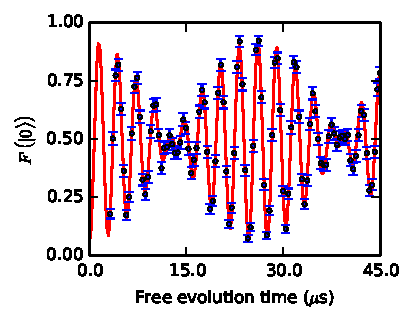
\includegraphics{Img/CarbonRamsey_C1.pdf}
    \caption{Uninitialized carbon-Ramsey of carbon-1.}
    \label{fig:CR_C1}
    \end{subfigure}
    \begin{subfigure}[t]{0.49\textwidth}\centering
        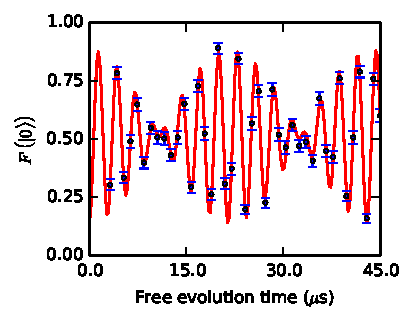
\includegraphics{Img/CarbonRamsey_C4.pdf}
        \caption{Uninitialized carbon-Ramsey of carbon-4.}
        \label{fig:CR_C4}
    \end{subfigure}
    \caption{The uninitialized carbon-Ramsey experiment shows an oscillation that is the sum of two cosines due to the phase picked up during free evolution.}
    \label{fig:Uninitialized_carbon_ramsey}
\end{figure}

\Cref{fig:Uninitialized_carbon_ramsey} shows the results for an uninitialized carbon-Ramsey experiment.
The data was fitted to a sum of two cosines in order to determine the frequencies.
% \begin{equation}
%     \left(A \cos(2\pi f_a \tau +\phi_a) + B \cos (2\pi f_b \tau +\phi_b)\right)/2 + a_0
%     \label{eq:carbon_ramsey_fitfunc}
% \end{equation}
The Larmor frequencies are $\omega_L = 2\pi\cdot 325.81 \pm 0.25$kHz  for carbon-1 and  $\omega_L =  2\pi\cdot 325.94 \pm 0.40$kHz for carbon-4.
Both the measured Larmor frequencies agree with the magnetic field of 304G within two standard deviations.

For $\tilde{\omega}$ the following frequencies were measured: $\tilde \omega= 2\pi\cdot 364.41 \pm 0.23$kHz for carbon-1
and $\tilde \omega = 2\pi\cdot 371.52 \pm 0.39 $kHz for carbon-4.
These frequencies can be used to disprove the estimations for the hyperfine parameters of \cref{tbl:HF_par}, however if the measured values agree with the hyperfine estimation we cannot conclude that they are correct.

Based on the estimated hyperfine parameters we expect $\tilde\omega =   \sqrt{(\omega_L+A_\parallel) ^2 + A_\perp^2}  \approx 364.7\mathrm{kHz}$ for carbon-1 and $\tilde \omega \approx 371.4 \mathrm{kHz}$ for carbon-4.
Both these values are in good agreement with experiment indicating that our hyperfine estimation is reasonably accurate. \footnote{Need a better sentence for this. }

\subsubsection{Measuring $T_{2,\mathrm{C}}^* $}
% Lange carbon ramseys van Hans sil01 140506 #53 en 56 +T2* analyse.
% hoeveel pulses voor de lange tau? belangrijk voor T2*
In order to know how many operations we can perform on a qubit we must know how long the signal stays coherent under normal operation.
In the case of controlling weakly carbons that is while decoupling the electron.

An uninitialized carbon-Ramsey experiment is performed with the small change that the electronic-spin is decoupled during the free-evolution time.
By undersampling with a frequency slightly offset from the precession frequency ($\omega_{\mathrm{DD}} = (\omega_L +\tilde{\omega} )/2$) a decaying cosine can be observed where the 1/e time of the envelope is equal to $T_2^*$.


\begin{figure}[htbp]
    \begin{subfigure}[t]{0.49\textwidth}\centering
    \includegraphics{Img/Carbon1_T2star.pdf}
    \caption{$T_2^*$-measurement for carbon 1.}
    \label{fig:T2star_carbon1}
    \end{subfigure}
    \begin{subfigure}[t]{0.49\textwidth}\centering
        \includegraphics{Img/Carbon4_T2star.pdf}
        \caption{$T_2^*$-measurement for carbon 4.   }
        \label{fig:T2star_carbon4}
    \end{subfigure}
    \caption{Carbon-Ramsey experiment to determine $T_2^*$ for nuclei while decoupling the electron. The decays are fitted with a generalized normal distribution to determine $T_2^*$ and the exponent $n$. For carbon-1, $T_{2,\mathrm{C}}^* =9.85 \pm   0.39 \mathrm{ms}$ and $n= 1.83 \pm 0.19$. For carbon-4,  $T_{2,\mathrm{C}}^* =6.68 \pm   0.22 \mathrm{ms}$ and $n= 2.31 \pm 0.31$. }
    % NOTE: Would like to add that it is not limited by electron coherence.
    \label{fig:T2star_carbon}
\end{figure}



Expected power N for ramsey type experiment
Expected T2 range ~ ms

Coherence time during operations/while addressing other gates.
Why electron decoherence is of no concern while determining T2* carbon?


\subsubsection{Single carbon tomography (ramsey met phase langs as en z init) }



\subsection{Controlling a single carbon}

\subsubsection{Theory, initialization and readout}

\subsubsection{Single qubit tomography and T2*}

\section{Controlling multiple-carbons}
\subsection{The parity measurement}
\subsection{MBE}

\begin{figure}[htbp]
    \centering
\mbox{
\Qcircuit @C=1em @R=.7em {
\lstick{\ket{0}_e} & \gate{\mathrm{y}}  & \ctrl{1} &  \ctrl{2} & \gate{y}  &  \meter &\qw\\
\lstick{\ket{0}_{C1}} & \qw&  \gate{\pm \mathrm{x}}  &\qw  & \qw       &\qw&\qw& \\
\lstick{\ket{0}_{C2}}& \qw& \qw  & \gate{\pm \mathrm{x}}    & \qw      &\qw&\qw&}}
    \caption{XX-parity-measurement}
    \label{fig:gate_circuit_XX-parity-measurement}
\end{figure}

\begin{figure}[htbp]
    \centering
\mbox{
\Qcircuit @C=1em @R=.7em {
\lstick{\ket{0}_e} & \gate{\mathrm{y}}  & \ctrl{1} &  \ctrl{2} & \gate{\mathrm{y}}  & \ctrl{1} &  \ctrl{2} &  \meter &\qw\\
\lstick{\ket{0}_{C1}} & \qw&  \gate{\pm \mathrm{x}}  &\qw  &\qw  & \gate{\pm \mathrm{x}} & \qw   &\qw&\qw& \\
\lstick{\ket{0}_{C2}}& \qw& \qw  & \gate{\pm \mathrm{x}}    & \qw    &\qw& \gate{\pm \mathrm{x}}    & \qw &\qw&}}
    \caption{General parity RO}
    \label{fig:gate_circuit_general_Parity_RO}
\end{figure}






\section{Controlling weakly coupled carbons trough the electronic spin}
% Section containing theory (Gate circuits) on how to initialize and readout carbons

Explain how carbon control works in theory.
Explain how a conditional and unconditional gate can be performed.
Explain initialization on gate level, refer to appendix for calculations.
Explain Readout.

\subsection{Initialized Carbon Ramsey}


\section{Carbon Initialization \& Readout}
% TODO_MAR: Discuss naming of sec: Carbon Init&RO and Carbon Tomo
%  Section containing experimental results (Tomographies)
%  Should emphasize difficulty in seperating initialization and RO fidelity, what is not working? Is it working?
Show results that demonstrate carbon control.



